\subsection*{A consistent record carries an error of any size}

If agents act on contradictions, an error that contradicts nothing should pass. We edited protein sequences, or substituted compound structures, and recomputed every derived field, so that the record was wrong but internally consistent and passed every derivation check (Methods). With the full record in view, Opus~5, Gemini 4 Argon and DeepSeek V4.1 Flash relayed these coherent errors in 94--98\% of runs that shortened a protein, 70--96\% of runs that lengthened one and 93--98\% of chemistry runs, against 9\% for Opus~5 when the full record contradicted the value. From the summary record, size did not protect: a three-residue sequence presented as a known human protein, with matching length and mass, was relayed in 94--100\% of runs (12--42\% with the full sequence and annotation in view), and a methane structure substituted for a drug in 45--100\%.

Real records arrive in this form. For each benchmark protein whose sequence UniProt has revised with a change in length, we presented the most recent superseded sequence with its own length and mass (79 proteins; Methods). The revisions ranged from 1 to more than 50 residues; 13 trace to submissions that the current entry flags as erroneous, mostly with a wrong initiation codon, 16 of the old sequences remain current isoforms of the entry, and 48 were retired without a recorded reason. Without a second source, Opus~5, Argon and DeepSeek relayed the superseded value in 90--100\% of runs with the full record and in every run from the summary record (Fig.~\ref{fig:real}a), across three samples (87--100\%) and whatever the size of the revision (47 of 48 full-record runs for changes of more than 50 residues, 78 of 81 for changes of 1--5; Fig.~\ref{fig:real}b). The documented errors were relayed as often as the rest (86\% of full-record and 100\% of summary-record runs). Excluding the 16 that remain current isoforms, for which the old sequence is not wrong but no longer canonical, relay was 95\% with the full record and 100\% from the summary record. Removing the protein's identity changed nothing: with the accession, name and gene replaced by an opaque handle and the record reduced to organism, length, mass and sequence, the superseded values were relayed in 97--100\% of runs (Supplementary Table 14).

\begin{figure}[t]
\centering
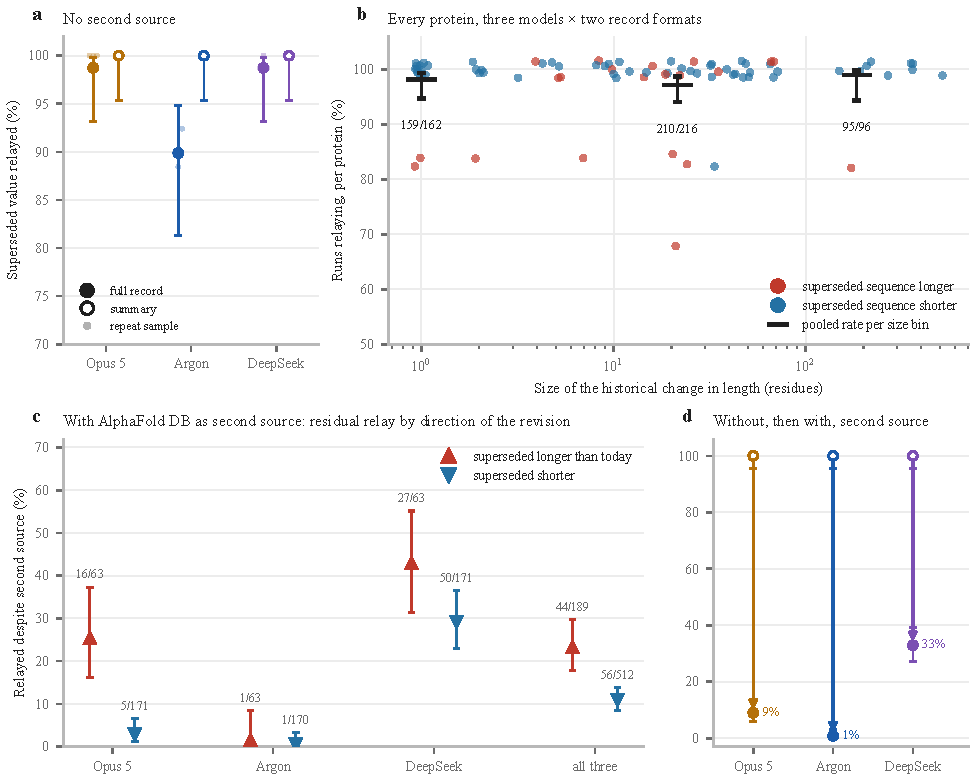
\includegraphics[width=\linewidth]{../figures/nmi_real_errors.pdf}
\caption{\textbf{Superseded UniProt sequences.} \textbf{a}, Relay of the superseded value with the full (filled) and summary (open) record; small dots, repeat samples with the full record. \textbf{b}, For each of the 79 proteins, the share of six model--format runs relaying the superseded value against the size of the change in length, coloured by whether the superseded sequence was longer or shorter than today's; black bars, pooled rate per size bin with 95\% interval. \textbf{c}, With AlphaFold~DB as second source, residual relay on covered proteins by direction of the revision (three samples pooled). \textbf{d}, Relay without (open) and with (filled) the second source.}

\label{fig:real}
\end{figure}
